%---------------Grundeinstellungen---------------------------------------------------------
\documentclass[a4paper,12pt, DIV12]{scrartcl}
% Trennungen, Schriftsatz; neue Deutsche Rechtschreibung
\usepackage[ngerman]{babel}
\usepackage[T1]{fontenc} % Umlaute, Sonderzeichen...
% Für Betriebssysteme mit utf8-Codierung
\usepackage{ucs}
\usepackage[utf8x]{inputenc} 
% ansonsten(z.B. Windows):
% \usepackage[ansinew]{inputenc}
%-----------------------------------------------------------------------------------------

%------------------Packete----------------------------------------------------------------
% Paket um Grafiken einzubinden. Evtl. muss unter Windows
% mit \usepackage[dvips]{graphicx} der dvips-Treiber für EPS-Grafiken geladen werden
\usepackage{graphicx}
\usepackage{subfigure}  % Bilder platzieren(z.B. nebeneinander)
\usepackage{multicol} % Paket für mehrspaltige Dokumente
\usepackage{float}    % Paket um Bilder in Fliess-Umgebungen einzubinden
\usepackage{amsmath}  % stellt die align-Umgebung zum Einrücken von Formeln zu Verfügung
\usepackage{amssymb}  % Extra mathematische Symbole
\usepackage{color}    % Farbdefinitionen
\usepackage{hyperref} % fuer klickbare Links
\usepackage{listings} % Quellcode farbig darstellen
\usepackage{lastpage} % Spezielles Paket um die Seiten zu zählen
\usepackage{scrpage2} % Kopf- und Fusszeilen
%\usepackage{pst-circ} % Elektronische Schaltungen
%\usepackage{pgfplots} % Für Diagramme
%----------------------------------------------------------------------------------------

%----------------Konfiguration-----------------------------------------------------------
\ihead{Inoffizielles Script zur Vorlesung Algebra 1, Prof. Schmidt}
%\chead{}
\ohead{Seite \thepage}
%\ifoot{}
\ofoot{Stand: \today}
%\cfoot{}
%\pagemark = Seitenzahl
\setheadsepline{1pt}    % Dicke der Trennlinie Kopfzeile - Text
\setfootsepline{0.5pt}  % Dicke der Trennlinie Fusszeile - Text
\pagestyle{scrheadings} % gemachte Einstellungen anwenden
\usepackage{setspace}   % Linienabstand
\onehalfspacing         % 1.5 Zeilenabstand; 1 = \singlespacing; 2 =
% \doublespacing
% schönere Hyperlinkfarben
\definecolor{darkred}{rgb}{0.5,0,0}
\definecolor{darkgreen}{rgb}{0,0.5,0}
\definecolor{darkblue}{rgb}{0,0,0.5}
\hypersetup{
  colorlinks,
  linkcolor=darkblue,
  filecolor=darkgreen,
  urlcolor=darkred,
  citecolor=darkblue
}
% Absatzeinzug
\setlength{\parindent}{0pt}  % Kein Einzug der ersten 1.Zeile eines Absatzes
% Verzeichnis in dem nach Bildern gesucht wird
% Sollte laut Dokumentation auch unter Windows/Mac gehen. Kann das jemand bestätigen?
\graphicspath{{bilder/}{:bilder:}}
%----------------------------------------------------------------------------------------

%----------------Beginn des eigentlichen Dokuments(also des Inhalts)---------------------
\begin{document}
\begin{titlepage}
\title{Inoffizielles Script zur Vorlesung Algebra 1 WS 2011 für IST, Prof. Schmidt}
% CS: Ich habe einfach mal die git Namen verwendet. Wer nicht drin stehen will, löscht sich halt wieder raus.
% Wir können auch Realnamen nehmen wenn ihr wollt. Meine commits sind ja eh immer mit dem vollen Namen ...
\author{Mitwirkende Autoren:\\
Mic92
\\
chaosbastler
\\
js75
}
\date{Revision: \today}
\maketitle

\begin{abstract}
Dieses Script wird fortlaufend mit den Vorlesungen erweitert. Es lohnt sich also ab und an nach Updates zu schauen.
\\Mitarbeit ist natürlich erwünscht, weitere Informationen auf der Projektseite: \url{https://github.com/Mic92/Algebra-I}
\end{abstract}
\end{titlepage}

\newpage
\tableofcontents
\newpage
\section{Mengen}
\subsection{Grundlegendes}
\subsubsection*{Was ist eine Menge?}
Eine Menge ist eine Zusammenfassung unterscheidbarer Objekte zu einer
Gesamtheit. Die Reihenfolge der Elemente ist irrelevant. Jedes Element ist
einzigartig.

Seien A und B Elemente, dann gilt:
\begin{align}
  A = B    &\Leftrightarrow \{A, B\} = \{A\} \\
  A \neq B &\Leftrightarrow \{A, B\} \neq \{A\}
\end{align}
D.h. gleiche Elemente werden in Mengen nur einmal gezählt.
2 Mengen sind genau dann gleich, wenn sie die selben Elemente
enthalten.
\subsubsection*{Besondere Mengen}
Die Menge, die keine Elemente enthält, wird als die \emph{leere Menge}
bezeichnet, das Symbol hierfür ist: $\{\}$ oder ${}\emptyset$.

Die \emph{Potenzmenge} ist die Vereinigung aller Teilmengen einer Menge.
Sie wird mit \(P(A)\) oder \(2^A\) bezeichnet. Jede Potenzmenge
enthält die leere Menge als Element.

\paragraph{Def.:} $P(A):= \{ U| {U}\subseteq{A} \}$
\paragraph{Beispiel:}
\begin{math}
{A = \{1,2,3\} }
\Rightarrow{2^A = \{ \emptyset, \{1\},\{2\},\{3\},\{1,2\},\{1,3\},\{2,3\}, A \} }
\end{math}
\newpage
\subsection{Mächtigkeit von Mengen}
Für endliche (abzählbare) Mengen ist die Mächtigkeit gleichzusetzen mit der Anzahl
der Elemente einer Menge. Für unendliche (nicht abzählbare) Mengen müssen andere
Definitionen getroffen werden, um deren Mächtigkeit zu beschreiben.
\paragraph{Man schreibt:}
\({}|{}A{}|{}\) oder \(\#A\)
\paragraph{Es gilt:}
\begin{math}
{}|{}2^A{}|{} = 2^{{}|{}A{}|{}}
\end{math}

\paragraph{Satz von Cantor}
Die Mächtigkeit der Potenzmenge einer Menge A ist stets größer als die Mächtigkeit der Menge A selber:
$$ |2^A| > |A| $$
Dies gilt insbesondere für die leere Menge, da $2^0>0$.
Außerdem ist für sämtliche endliche Mengen klar: $ 2^n > n $.  Auch bei unendlichen Mengen lässt sich die Gültigkeit des Satzes zeigen.

\subsubsection*{Gleichmächtigkeit}
Seien A und B zwei beliebige Mengen.
Dann heißt A gleichmächtig zur Menge B, wenn eine Bijektion (\({f:A}\rightarrow{B}\)) gebildet
werden kann. Das bedeutet, dass eine Vorschrift existiert, welches
jedem Element der Menge A genau ein Element der Menge B zuordnet.
Dabei werden alle Elemente der Menge B einmal erfasst. Diese
Vorschrift ist umkehrbar.
\paragraph{Man schreibt:} \(\#A = \#B\) bzw. \(|A| = |B|\)
\paragraph*{Beispiele:}
\begin{math}
\#{\mathbb N} = \#{\mathbb Z} = \#{\mathbb Q}
\end{math}

Jede Menge, die gleichmächtig zur Menge der natürlichen Zahlen ist, wird als \emph{abzählbar} bezeichnet.
Die Mächtigkeit der reelen Zahlen hingegen wird als \emph{überabzählbar} bezeichnet.
\subparagraph{Erläuterung zu \(\#{\mathbb N} = \#{\mathbb Z}\):}
\begin{figure}[b]
  \centering
  \caption{Beispiel für eine Abbildung \(\#{\mathbb N} = \#{\mathbb Z}\)}
  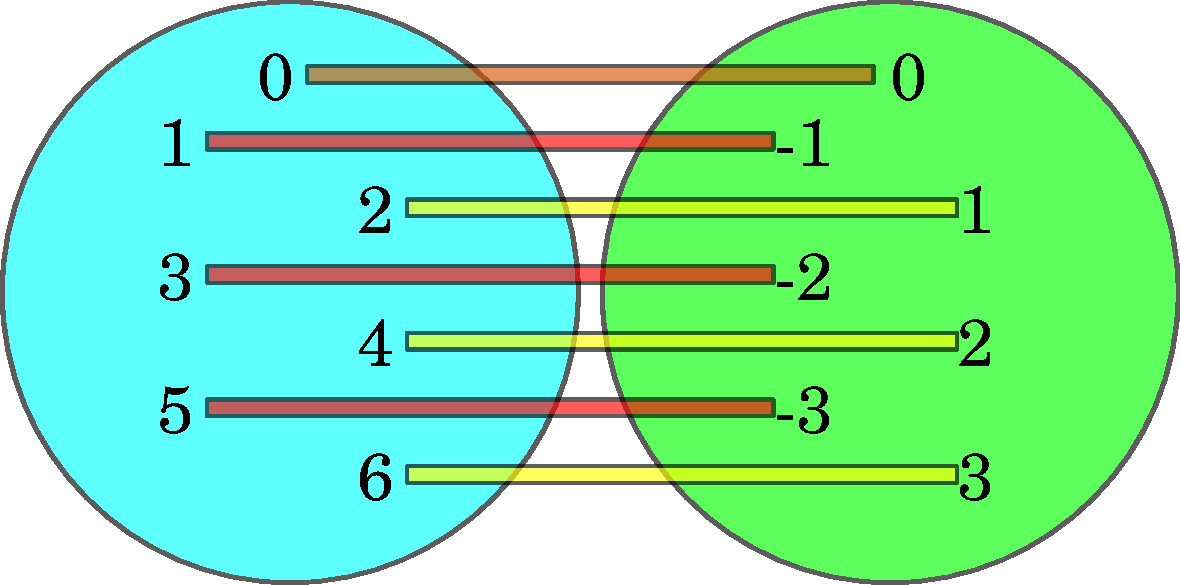
\includegraphics[scale=0.5]{ngleichz.pdf}
\end{figure}
Der Einwand, dass die natürlichen Zahlen doch ``offensichtlich'' (von der 0
abgesehen) doppelt so viele seien müssten, wie die ganzen Zahlen zählt
bei diesen unendlichen Mengen nicht! Stattdessen sollte man an die
Definition der Gleichmächtigkeit denken: 2 Mengen sind dann gleich,
wenn es eine eineindeutige(bijektive) Abbildung gibt.
Es werden also die 0 auf die 0, die ungeraden Zahlen auf die positiven
Zahlen und die geraden Zahlen auf die negativen Zahlen abgebildet.
Dies ist aufgrund der Unendlichkeit der beiden Mengen ohne Probleme
möglich.

Auch für die rationalen Zahlen lässt sich ein solches Schema für eine Bijektion finden.
Hierauf geht ein Wikipedia-Artikel näher ein:

% J.S.: Wir sollten die Wikipedia-Artikel später in das Skript einarbeiten..
\url{http://de.wikipedia.org/wiki/Cantors_erstes_Diagonalargument}

Und auch bei der Frage, warum die reellen Zahlen nicht abzählbar sind, hilft Wikipedia:

\url{http://de.wikipedia.org/wiki/Cantors_zweites_Diagonalargument}

% Quelle für nächsten Abschnitt: Repetorium höhere Mathematik, Merziger, Wirt, 6. Auflage, S.41 Aufgabe 1.60 und Lösung dazu
\subparagraph{Beispiel für überabzählbare Mengen}
Ähnlich wie beim vorherige Beispiel widerspricht es auch der Intuition, dass die Menge $\{ x | x \in (0,1) \}$ sowie $\{x | x \in {\mathbb R} \}$ gleichmächtig sind.
Schließlich ist das Intervall $(0,1)$ ja nur eine Teilmenge der reelen Zahlen.
\\Tatsächlich kann man schon mit Schulmathematik eine solche Bijektion finden: $$ f(x) = {1}/{\pi} * (arctan(x) + \pi/2 ) $$
Wer einen Blick auf den Graphen von $arctan(x)$ wirft wird dies schnell einsehen: 
die Funktion durchläuft sämtliche Werte von $-\infty$ bis $\infty$ und nimmt dabei nur Werte von $-\pi/2$ bis $\pi/2$ an. 
Durch Stauchung mit dem Faktor ${1}/{\pi}$ sowie Verschiebung nach oben kommt man dann zu obiger Funktion.

%%% Local Variables:
%%% mode: latex
%%% TeX-master: "../script"
%%% End:

\newpage
\section{Abbildungen}
\subsection{Definition}
Seien A und B zwei Mengen.
Dann ist eine \emph{Abbildung} ein eindeutige Vorschrift, die jedem Element aus A genau ein Element aus B zuordnet.
Ein andere Bezeichnung für Abbildung ist \emph{Funktion}.

Die Menge $A$ wird als \emph{Definitionsbereich} bezeichnet.

Die Menge $B$ wird als \emph{Wertebereich} bezeichnet.

Der \emph{Bildbereich} wird definiert als
$ f^{ [A] }:=\{b | b=f(a) , a \in A \}$.
Er ist Untermenge des \emph{Wertebereichs}. Bei surjektiven Abbildungen
ist der Bildbereich gleich dem Definitionsbereich.

Von bijektiven Funktionen kann eine \emph{Umkehrfunktion} $f^{-1} :
{B}\rightarrow{A} $ gebildet werden. Deswegen bezeichnet bijektive
Funktionen auch als \emph{invertierbar}.

Diese ist nicht zu verwechseln mit dem \emph{Urbild}, was ähnlich geschrieben wird.

\subsubsection*{Beispiel}
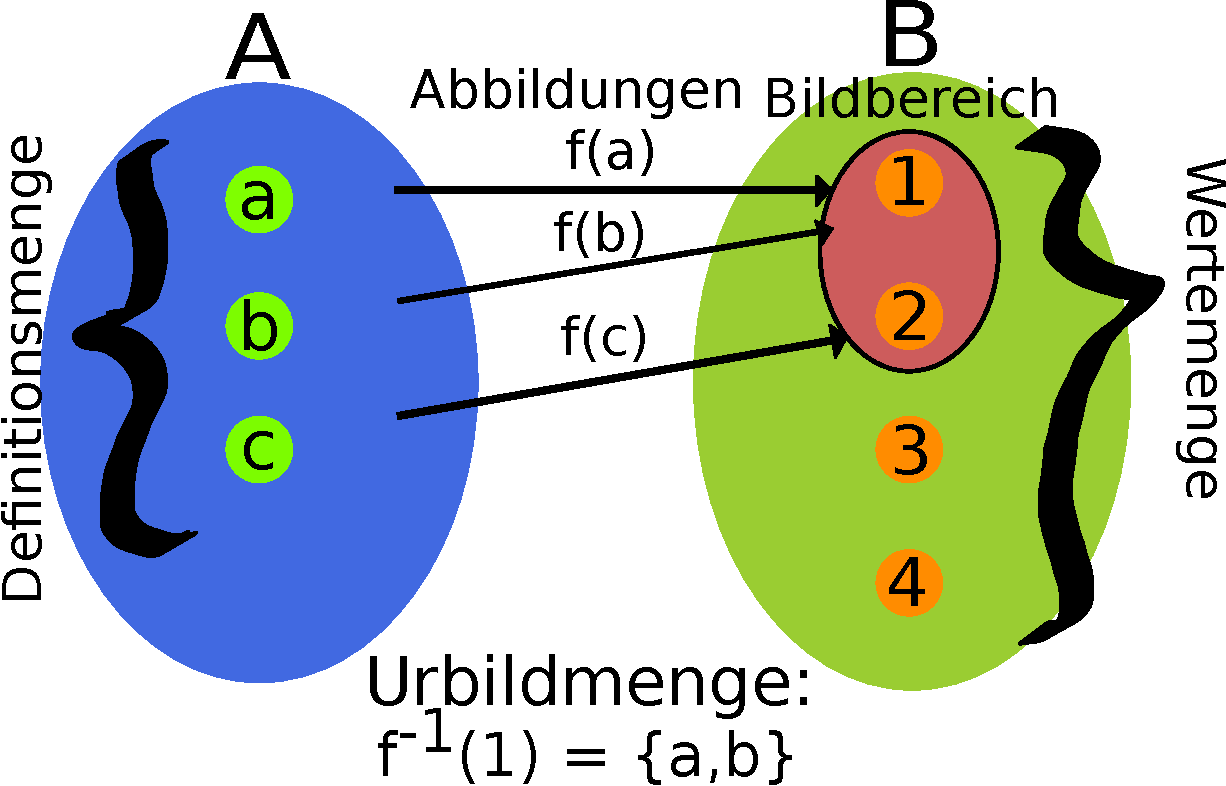
\includegraphics[scale=0.5]{abbildung.pdf}
%%% Local Variables:
%%% mode: latex
%%% TeX-master: "../script"
%%% End:

\newpage
\subsection{Kern einer Funktion}
Sei $f:{A}\longrightarrow{B}$ eine Abbildungsvorschrift.
Dann ist:
\begin{align*}
   \ker(f) := \{(a,b) | f(a)=f(b)\} %Interessant: \ker ist bereits definiert!
\end{align*}
eine Menge, der sogenannte Kern von f.
\subsubsection{Beispiel}
\begin{align*}
  f: &\mathbb{R} \rightarrow \mathbb{R} : {x}\longmapsto{x^2} \\
  \ker(f) &= \{(a,b) | f(a)=f(b) \} \\
         &= \{ (a,b) | a^2 = b^2 \} \\
         &= \{ (a,b) | |a| =|b| \}
\end{align*}

% Brauch mein Emacs um das Masterfile zu finden
%%% Local Variables:
%%% mode: latex
%%% TeX-master: "../script"
%%% End:

\newpage
%*********************************************************
% Änderung vom 09.11.11: Bisherige Definition entfernt und durch
% Definition von Prof. Schmidt ersetzt. (js75)
% chaosbastler: die Schreibweise mit Quantoren fand ich Übersichtlicher als Text ...
% Außerdem war die alte Version mit der Fettsschreibung von ``surjektive Abbildung' usw. auch etwas übersichtlicher
%*********************************************************
\subsection{Typen von Abbildungen}\label{kap_typabb}
\subsubsection{Definition}
\begin{description}
\item Eine Abbildung $f \colon A \rightarrow B$ heiße \emph{injektiv} falls für
$a, b \in X$ aus $x \neq t$ stets $fx \neq ft$ folgt (es gibt also keine Kollisionen).
\item Es heiße $f$ \emph{surjektiv}, falls zu jedem $y \in B$ ein $x \in A$
existiert mit $fx = y$ (es wird also jedes Element der Zielmenge abgedeckt).
\item Ferner heiße $f$ \emph{bijektiv}, falls $f$ injektiv und surjektiv ist.
\end{description}
Ist $f \colon A \rightarrow B$ eine Abbildung, so sei für $X \subseteq A$ stets
$fX \coloneq f[X] \coloneq \{fx | x \in X\}$ die Menge der Bilder von $X$ unter
$f$.

Ferner heiße $\text{Bild}(f) = \text{Im}(f) \coloneq fA$ die
\emph{Bildmenge}\footnote{Bild = Image} von $f$. $f$ ist genau dann surjektiv,
wenn (gdw\footnote{im englischen Sprachraum \emph{iff} = if and only if}) $fA = B$
gilt, das heißt die Bildmenge von $f$ ist gleich der Zielmenge von $f$. Daraus
folgt: $fX \subseteq fA$

\subsubsection{Bezeichnungen}
\begin{description}
\item Sind $A$ und $B$ Mengen, so bezeichnen $B^A \coloneq \text{Abb}(A,B)
\coloneq \text{Map}(A,B)$ die Menge aller Abbildungen von $A$ nach $B$.
\item $\text{Surj}(A,B)$ sei die Menge aller surjektiven Abbildungen
(\emph{Surjektionen}) von $A$ nach $B$,
\item $\text{Inj}(A,B)$ sei die Menge aller injektiven Abbildungen
(\emph{Injektionen}) von $A$ nach $B$,
\item $\text{Bij}(A,B)$ sei die Menge aller bijektiven Abbildungen
(\emph{Bijektionen}) von $A$ nach $B$.
\end{description}

\begin{figure}
\subfigure[surjektive
Abbildung]{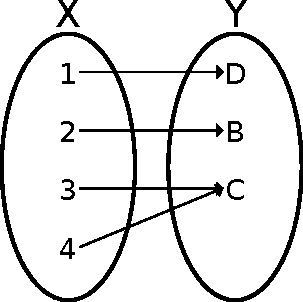
\includegraphics[width=3cm]{Surjection.pdf}}\hfill
\subfigure[injektive
Abbildung]{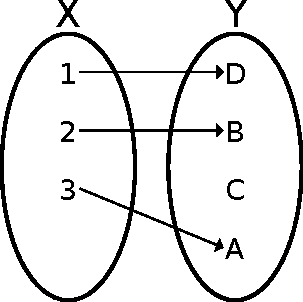
\includegraphics[width=3cm]{Injection.pdf}}\hfill
\subfigure[bijektive
Abbildungen]{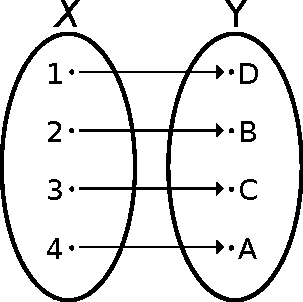
\includegraphics[width=3cm]{Bijection.pdf}}\hfill
\subfigure[identische
Abbildungen]{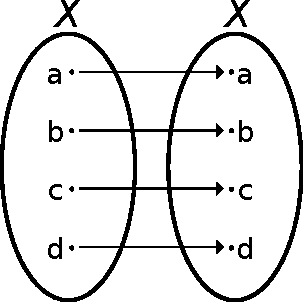
\includegraphics[width=3cm]{Identitaet.pdf}}
\end{figure}

\subsubsection{Mächtigkeit von Definitions- und Wertebereich}

Für Surjektionen gilt: $|A| \geq |B|$

Für Injektionen gilt: $|B| \geq |A|$

Weil für bijektive Abbildungen beide Aussagen gelten müssen gilt:
$$|A| \geq |B| \wedge |B| \geq |A| \Rightarrow |A| = |B| $$


Analog gilt auch:
$$ |A|<|B| \Longleftrightarrow Surj(A,B) = \emptyset $$
$$ |A|>|B| \Longleftrightarrow Inj(A,B) = \emptyset $$
$$ |A| \neq |B| \Longleftrightarrow Bij(A,B) = \emptyset $$

Die ersten Aussagen schließen von einem Typ von Abbildung auf die Mächtigkeit von Definitions- und Wertebereich.
Die drei letzen Aussagen schließen von Definitions- und Wertebereich auf die (nicht) möglichen Typen von Abbildungen.

Würden die Beziehungen zwischen den Mächtigkeiten nicht gelten, würde z.B. die Formel zur Mächtigkeit von Inj(A,B) zu Widersprüchen führen(vlg. nächstes Kapitel).
\newpage
\subsection{Mächtigkeit von Mengen von Abbildung}
Seien $A$ und $B$ Mengen.
Dann bezeichnet $B^A$ oder $\Map(A,B)$ die Menge aller Abbildungen von $A$
nach $B$. \paragraph*{Satz:}
Für $A, B$ endliche Mengen gilt:
$$ |B^A| = {|B|}^{|A|} $$

\paragraph*{bijektive Abbildungen}
Sei $|A|=|B|$ endlich. Die Mächtigkeit der Menge aller bijektiven
Abbildungen von A nach B entspricht der Anzahl der Permutationen auf
einer |A|-elementigen Menge.
\begin{align*}
  A &\rightarrow B \\
  (|A|)! &= (|B|)!
\end{align*}

\paragraph*{injektive Abbildungen}
Seien |A| und |B| endlich. Die Mächtigkeit der Menge aller injektiven
Abbildungen von A nach B entspricht einer \emph{Variation} ohne Zurücklegen:
\begin{align*}
  A &\rightarrow B \\
  a &= |A| \; b = |B| \\
  {{b}\choose{a}} * a!
  &= \frac{b!}{(b-a)!}
\end{align*}

\subparagraph*{Anmerkung:} Für den Sonderfall $|A|=|B|$ führt die Formel auf die Formel für die bijektiven Abbildungen zurück. Das bedeutet, dass im Fall $|A|=|B|$ endlich jede Injektion
automatisch auch eine Bijektion ist.

\paragraph*{surjektive Abbildung}
Seien |A| und |B| endlich. Die Mächtigkeit der Menge aller surjektiven
Abbildungen von A nach B lässt sich mithilfe der
Stirlingzahl 2. Art ($S_{n,r}$) berechnen.
\begin{align*}
  A &\rightarrow B \\
  a &= |A| \; b = |B| \\
  b!    &\cdot S_{(a,b)}\\
  S(a,b)&=\frac{1}{b!}\sum_{j=1}^{b}(-1)^{b-j}{b \choose j}j^a
\end{align*}

\subparagraph*{Bemerkung:} Die Formel für surjektive Abbildung sollte als Ergänzung zum Vorlesungsstoff verstanden werden. 
Sie wird(soweit wir bisher wissen) nicht als bekannt vorrausgesetzt.

\end{document}
